\documentclass[3p,twocolumn]{elsarticle}
%%\usepackage[utf8]{inputenc}
%%\usepackage[LGR,T1]{fontenc}
%%\usepackage{graphicx,amsmath}
%%\usepackage[british]{babel}
%%\usepackage[latin9]{inputenc}%SOME KIND OF CLASH WITH THIS ONE
%%\usepackage{array}
%%\usepackage{rotfloat}
%%\usepackage{textcomp}
%%\usepackage{amssymb}
\usepackage{amsmath} 
%% to align equations \usepackage{mathrsfs} % curly font in math, called using mathscr
%%\usepackage{graphicx}
%%\usepackage{subcaption} % to have two images under one caption
%%\usepackage{subscript}
%%\usepackage{gensymb} %for degree symbol
\setlength{\marginparwidth}{2cm} % to set the width of the marginpar
\usepackage{todonotes}
%%\usepackage{xargs}                      % Use more than one optional parameter in a new commands
%%\renewcommand{\baselinestretch}{1.5}
\bibliographystyle{elsarticle-num}
\begin{document}
\begin{frontmatter}
\title{Advanced Characterisation of Pore Structure in Next-Generation Reactor Graphites}
\author[plym]{Bradley Moresby-White}
\author[plym]{Katie L. Jones\corref{cor1}}
\ead{katie.jones@plymouth.ac.uk}
\author[plym]{G. Peter Matthews}
\author[plym]{Giuliano M. Laudone}
\cortext[cor1]{Corresponding author.}
\address[plym]{Faculty of Science and Engineering, University of Plymouth, Plymouth, UK}
\begin{abstract}
Nuclear grade graphite
\end{abstract}
\begin{keyword}keyword\sep keyword\sep keyword\end{keyword}
\end{frontmatter}
\section{Introduction}
\section{Methodology}

\subsection{Materials}

Virgin graphite samples of two grades, IG-110 and IG-430, were supplied by Toyo
Tanso Ltd\texttrademark{}, Osaka, Japan. The properties of both grades are
tabulated (Table ~\ref{tab:materialstable}).IG‑110 is currently employed in the
three existing HTGRs worldwide, while IG‑430 is designed to deliver increased
density, strength, and thermal conductivity for future
applications.\citep{toyotanso_atomic_nuclear} (Table ~\ref{tab:materialstable}).
Both grades comply with \textit{ASTMD7219-19}, including the requirement for a
minimum bulk density exceeding 1.7 g/cm$^3$ \citep{ASTMD7219-19}
(Table~\ref{tab:materialstable}). \todo{Is this necessary? I do like it, talking about the
  standards, but it is a bit of a tangent.}
\todo{for the following table, better to directly cite the manuf?}
\begin{table*}
  \centering
  \caption{Manufacturer dataset for IG-110 and IG-430 \citep{Jones2018}}
  \label{tab:materialstable}
  \resizebox{\textwidth}{!}{%
    \begin{tabular}{l l c c c c c}
      \hline
      Grade   & Coke source & Bulk density/g cm$^3$ & Filler particle size/$\mu$m) & Tensile strength/MPa & Young's modulus/GPa & Thermal conductivity/W m$^{-1}$K$^{-1}$\\
      \hline
      IG‑110  & Petrol    1        & 1.77                  & 10                           & 25                     & 9.8                   & 120 \\
      IG‑430  & Pitch             & 1.82                  & 10                           & 37                     & 10.8                  & 140 \\
      \hline
    \end{tabular}%
  }
\end{table*}

\subsection{Sample preparation}
Cuboids were sub-sampled from the virgin graphite blocks, with dimensions of
approximately 10mm x 10mm x 100mm. The sub-samples were further subsampled into
cuboids of side lengths ~7mm, providing 3 cuboids per grade. Samples were
polished via SiC polishing pads up to a grit size of P5000, to minimise
topographical variations induced by sample preparation that may cause artefacts
during either SEM imaging or low pressure gas adsorption \citep{Fang2022,Jones2018}.
Samples were sonicated in 2-propanol for 24h to remove any contaminants,
including the lubricant used in the machining process or silica particles
introduced during polishing. Samples were then dried under vacuum for 12 h at
$305 \pm 5\,^\circ\mathrm{C}$ using the BELPREP-vac (MicrotracBEL, Japan) in
order to remove any residual moisture introduced during the sonication process.

\todo{Could talk here about how we wanted to do resin impeg like Kane et al, but
  did not have the chance, and explain this might introduce issues, also we
  could talk about how this is quite rough, and that this kind of sample
  preparation (i.e. no vibratory polishing, no resin impregnation) is not ideal
  and may have introduced both artefacts and noise. Additionally, sonication may
  have damaged the pore structure}

\subsection{Scanning Electron Microscopy (SEM)}

SEM microscopy fundamentally consists of an electron source, confined to a thin
beam, accelerated towards the sample. The resulting electrons strike the
photomultiplier, generating electrical signals that are subsequently amplified
\cite{Achaw12, Goldstein2003}. For SEM analysis of the surface features of
nuclear-grade graphite, the signal of interest is the secondary electrons, which
are produced when the incident electrons from the beam excite electrons within
the atoms of the graphite surface. These excited electrons migrate toward the
surface and only escape if they possess sufficient energy to overcome the
material's work function \cite{Achaw12, Goldstein2003}. Given the low
accelerating voltage applied in this work (5 kV), only the secondary electrons
representing the first few nanometers of the sample surface can exit and be
detected \cite{Achaw12, Goldstein2003}.

The construction of the micrographs is the result of signal amplification from
the secondary electrons via the photomultiplier tube, which generates a
two-dimensional intensity distribution represented as micrographs. This process
yields a high-quality representation of the sample surface topography. The
JEOL\texttrademark IT510 Scanning Electron Microscope was employed to generate
the contiguous set of individual micrographs from which the full composite
micrograph was assembled. The Image Montage capability within the JEOLInScope™
package performed this function. The system captures multiple micrographs by
using a motorized stage to move the electron beam over the specified area with a
set overlap for each new micrograph. The software automatically adjusts
stigmation, contrast, and brightness. Analysis of the metadata for all 1,350
micrographs demonstrated that shifts in contrast and brightness were minor,
having a negligible impact therefore on the later selection of the intensity
threshold for the full composite (Table ~\ref{tab:contrast-brightness-summary})
The complete set of selected parameters is tabulated in Table
~\ref{tab:microscopy_parameters}.

\begin{table}[ht]
  \centering
  \caption{Contrast (C) and Brightness (C) Summary by Sammple}
  \label{tab:contrast-brightness-summary}
  \resizebox{\columnwidth}{!}{%
  \begin{tabular}{lrrrr}
    \hline
    Variant & Avg C (\%) & Std C (\%) & Avg B (\%) & Std B (\%) \\
    \hline
    IG430B & 98.01 & 1.02 & 99.69 & 0.08 \\
    IG430C & 98.16 & 0.82 & 99.83 & 0.08 \\
    IG110B & 95.86 & 0.72 & 99.26 & 0.13 \\
    IG110C & 94.03 & 0.93 & 99.38 & 0.13 \\
    IG110F & 98.20 & 0.70 & 99.69 & 0.13 \\
    \hline
  \end{tabular}
  }
\end{table}

\begin{table}
  \centering
  \caption{Parameters for composite assembly captured with the JEOL IT510 SEM using Image Montage Mode}
  \label{tab:microscopy_parameters}
  \begin{tabular}{l l}
    \hline
    Parameters & Values \\
    \hline
    Magnification ($\times$)                    & 1000 \\
    Resolution ($\mu$m/px)               & 0.1 \\
    Surface area per micrograph ($\mu$m$^2$) & 12\,288 \\
    Overlap (\%)                          & 10 \\
    Micrographs per sample (n)            & 196 \\
    \hline
  \end{tabular}%
\end{table}

In this work, a magnification of 1000X was selected as an optimal compromise
between the resolution necessary for capturing the pore structure at the
required scale and the total area covered by each micrograph. The scale of this
study is significant, with each micrograph covering 12,288 µm² and each sample
consisting of 225 micrographs, yielding a total imaging area of 2.765 mm² per
sample. With 3 samples analysed per grade, the total scanned area per graphite grade is
8.294 mm². Given this scale, each composite micrograph represents a substantial
section of the sample and captures a thousands of pores.
\todo{Huang 2021 used 5000× magnification with 48 micrographs per sample, covering 0.13 mm × 0.13 mm for their composite.}
\todo{I actually did 0-14 so that is 15 x 15 which is 225 micrographs per sample, not 196.}

\subsection{Composite assembly}

The composite assembly stage ("stitching") , where the overlapping micrographs
are combined into a single image per sample, may have a significant impact on
the porosity values generated as incorrect fusion will misrepresent pore
structures. To address this, a stitching method based on the phase correlation
approach developed by Kuglin and Hines (1975) and further refined by Preibisch
et al. (2009) was employed as an ImageJ plugin \citep{Kuglin1975,
Preibisch2009}.
	
One advantage of this method is the avoidance of error propogation by
consecutive registration steps, as simply placing micrograph A relative to
micrograph B, and then micrograph B relative to micrograph C, would result in
accumulation of errors. This method builds a graph whose nodes are the
micrographs, and edges are the measured pairwise shifts between the micrographs.
It then finds the set of micrograph positions that minimize the total squared
registration error across the entire graph, a form of globally optimized
registration \citep{Preibisch2009}.

This stitching method also allows sub-pixel accuracy, which is crucial for
accurate pore measurement. If each micrograph is a discrete 2D signal, then for
any two micrographs \(A\) and \(B\), which are shifted relative to each other
(i.e., micrograph \(B\) is shifted two pixels up and 10 pixels left of
micrograph \(A\) ) then their Fourier transforms would have the same magnitude
but different phases. A normalized cross-power spectrum isolates the phase
difference, and from there the Inverse Fourier transform yields a correlation
map with peaks indicating possible translations between the micrographs.
Unfortunately, complexity of real images and the periodicity of the Fourier
transform means that the correlation map is not a single peak, but rather a set
of peaks, each representing a possible translation. This method therefore
selects the \(n\) highest local maxima and finds the peak with the best
correlation, which it defines as the true translation between the two
micrographs \citep{Preibisch2009}. Finally, sub-pixel accuracy in that shift is
achieved by applying a parabolic interpolation around the selected peak to
refine the translation estimate.

Additionally, a non-linear intensity blending function eliminates the visible
seams between micrographs, which can occur even when the micrographs are
perfectly aligned due to shading variations. This blending assigns a weight to
each pixel in a tile, working as a function of the distance from the tile edge,
with the a tunable parameter controlling this weighting function. In
non-overlapping regions, the centre of the micrograph, the weight is essentially
1, so the original pixel value is preserved exactly. In overlapping regions,
intensities are a convex combination of the original values. Crucially, because
the weights sum to 1 everywhere, blended intensity is simply a weighted average
of the original intensities. Thus, the final composite micrograph is still a
valid representation of the original micrographs, but the seams have been
removed, and the transition between micrographs is smooth \citep{Preibisch2009)}.
Testing indicated that different values in the blending parameter, which is
tunable, had no discernable impact on the final composite micrograph, and
therefore no impact on the final porosity values. By contrast, the removal of the
visible seams between micrographs did increase confidence that in the following
steps, the subsample used to determine the intensity threshold was
representative of the full composite micrograph.

The resulting composite micrographs showed excellent alignment with no visible
delineation between individual micrographs, a total area comparable with
previous works, high resolution, and clear distinction between porosity and bulk
when examined closely (Figure \ref{fig:IG430C split scaled}
\cite{Huang2019,Kane2011a}). 

	\begin{figure}
		\centering
		\includegraphics[width=0.45\textwidth]{./Media/C1-IG430c fusion cropped split scaled.jpg}
		\caption{Fully assembled SEM composite: IG-430 Sample C, 1000×  magnification,
     5 kV accelerating voltage. Bar = 250 µm.}
		\label{fig:IG430C split scaled}
	\end{figure} 

	\subsection{Computation of Channel Porosity}
\subsubsection{Intensity/Greyscale Thresholding}

For each 8-bit micrograph \(E\) (pixel values \(0 \le E(x,y) \le 255\)), we
first compute its intensity histogram \(H(i)\) for \(i=0,1,\dots,255\).
Specifically,
\[
H(i) = \sum_{x=1}^{M}\sum_{y=1}^{N} \mathbf{1}\{E(x,y)=i\},
\]
where \(M\) and \(N\) are the image width and height (in pixels), and
\[
\mathbf{1}\{E(x,y)=i\} =
\begin{cases}
1, & \text{if the pixel at }(x,y)\text{ has intensity }i,\\
0, & \text{otherwise.}
\end{cases}
\]

The indicator function \(\mathbf{1}\{E(x,y)=i\}\) “tests” each pixel, yielding 1
if the pixel greyscale value equals \(i\) (e.g. greyscale value of 250), and 0
otherwise. The double sum \(\sum_{x=1}^M\sum_{y=1}^N\) runs that test over every
pixel in the micrograph resulting in a histogram \(H(i)\) of 256 bins, each bin
representing number of pixels in the micrograph at each greyscale value \(i\). 

Intensity thresholding then \(H(i)\) determines a greyscale value
at which porosity and bulk (i.e., foregound and background) are distinguished.

Global automatic thresholding algorithms optimise by different
criteria (i.e. maximisation of inter-class variance, minimisation of
intra-class variance) to determine thresholds. For manual selection of a given
threshold, or validation of an automatically selected threshold, there exists
no certain criteria to allow a fully objective evaluation
\citep{Huang2019}.Thresholding aims to select an intensity value that reliably
binarizes porosity and bulk in a way that minimizes both Type I and II errors,
as evaluated by the operator (i.e., false positives, classifying a pore where
one is not present, and false negatives, not classifying a pore where one is
present).

A test of all 17 of the available automatic thresholding methods available in
ImageJ demonstrated that none of the avilable automatic global intensity
thresholding algorithm effectively distinguished between porosity and bulk
with the sensitivity required to allow the classification of pores for the
given histogram (Figure ~\ref{fig:Try All Thresholding Methods}). The key
cause is likely the lack of a bimodal distribution in the histograms generated
by any of the micrographs , meaning that there are statistically no classes to
be separated (Figure ~\ref{fig:histogramnobimodal}). 

    \begin{figure}
		\centering
    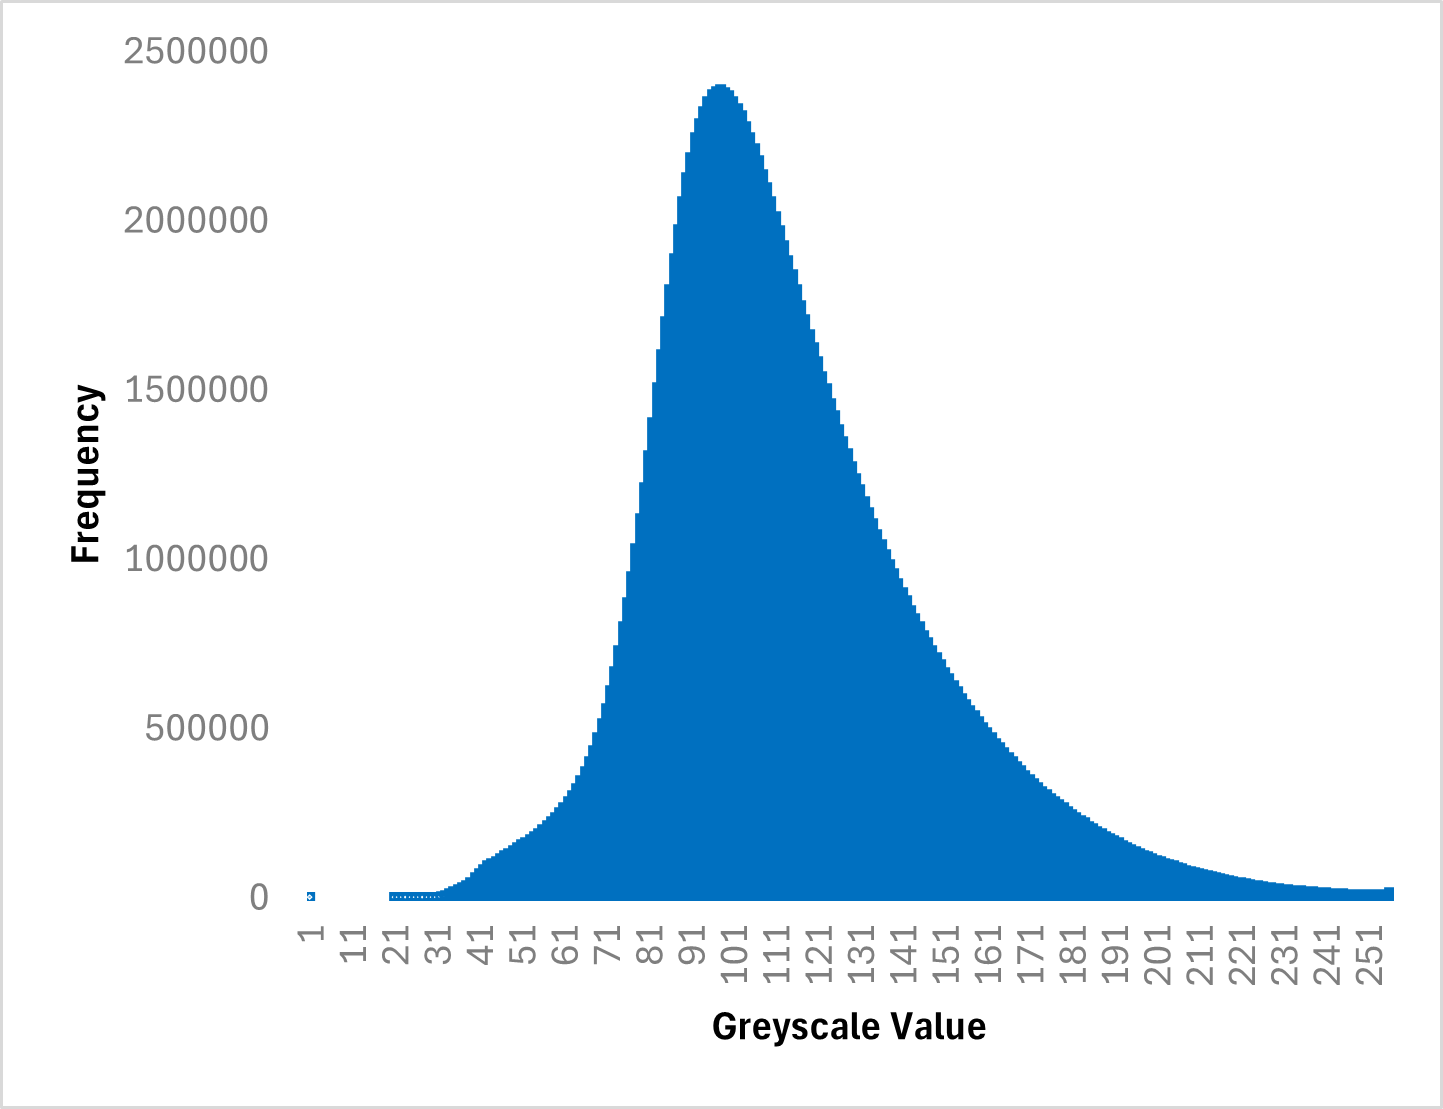
\includegraphics[width=0.45\textwidth]{./Media/IG430F Greyscale Histogram.png}
		\caption{PLACEHOLDER DRAFT: Histogram of greyscale values for IG-430 Sample F, 1000×, Showing skewness and unimodality}
		\label{fig:histogramnobimodal}
	\end{figure} 

	\begin{figure}[!htbp]
		\centering
		\includegraphics[width=0.45\textwidth]{./Media/MontageIG430C Methods.jpg}
		\caption{Thresholded Micrograph of IG-430 Sample C at $1000\times$ Magnification. Methods are placed sequentially from right to left, row by row. 
    (a) Default
			(b) Huang
			(c) Huang2
			(d) Intermodes
			(e) IsoData
			(f) Li
			(g) MaxEntropy
			(h) Mean
			(i) MinError(I)
			(j) Minimum
			(k) Moments
			(l) Otsu
			(m) Percentile
			(n) RenyiEntropy
			(o) Shanbhag
			(p) Triangle
			(q) Yen}
		\label{fig:Try All Thresholding Methods}
	\end{figure}  

	A HITL (human in the loop) approach was therefore undertaken, as illustrated
	in the  process diagram (Figure ~\ref{fig:Final Workflow}). Here, the operator
	subsamples the composite micrograph, then examines this subsample to
	determine the threshold at which porosity and bulk are best separated. The
	operator then applies this threshold, along with a pore diameter threshold, to
	the full composite. The composite micrograph has therefore been binarized and 
  porosity can be quantified via various connected component analysis
  algorithms, such as the "Analyse Particles" function in ImageJ.

\begin{figure}[!htbp]
    \centering
    \includegraphics[width=0.45\textwidth]{./Media/Newprocessmodel.png}
    \caption{Full thresholding workflow detailing the process of micrograph generation,
     composite assembly, subsampling, intensity thresholding, and pore diameter thresholding.}
    \label{fig:Final Workflow}
\end{figure}

An output from this process is exemplified, selected at random, which demonstrates excellent delinieation 
of pores, according to an inevitably subjective operator evaluation (Figure ~\ref{fig:dualintensitythreshig430f}).

\begin{figure}[!htbp]
    \centering
    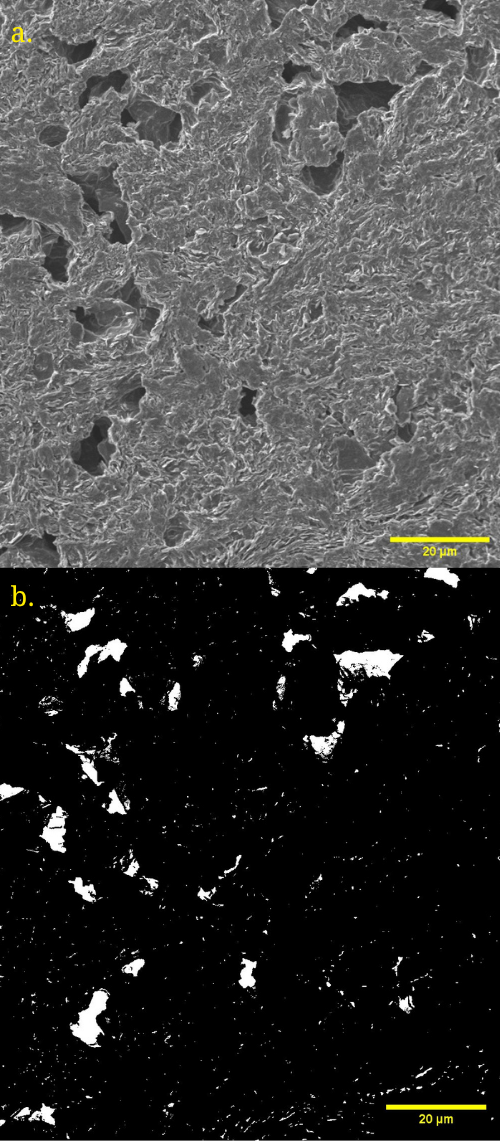
\includegraphics[width=0.45\textwidth]{./Media/intensitythresholdexampleig430fdual.png}
    \caption{DRAFT: IG430F raw (a) and following intensiy thresholding (b)}
    \label{fig:dualintensitythreshig430f}
\end{figure}

	\subsubsection{Pore Diameter Thresholding}
    
  Pore size thresholds were imposed in this work, as in previous studies
  \citep{Taylor2016, Huang2019, Kane2011a}, to restrict the automated
  recognition of pores to a range (i.e., only counting pores > 12.5µm\(^2\))
  where classification is deemed reliable. However, this approach is inherently
  limited by the practical difficulty of objectively determining whether any
  given pore classification is correct.
      
  As shown in (Table ~\ref{tab:thresholdsandvariationsIG430F}), extreme changes
  in the total pore count result from minor alterations in the threshold, with a
  0.5 µm\(^2\) threshold yielding a total pore count of 11,375, while a 1
  µm\(^2\) threshold yields a pore count of 6,485. Crucially however the total
  area of pores above the threshold remains relatively stable, with a porosity
  of 3.8\% for the 0.5 µm\(^2\) threshold, and 3.6\% for the 1 µm\(^2\)
  threshold. When combined with individual analyses of the resulting PSDs and
  precise examination of exactly which features are excluded at each threshold
  as per (Figure ~\ref{fig:improvedporediademo}), a pore area threshold of 1
  µm\(^2\) (dia = 1.12 µm) was selected an optimal compromise between type I and
  II errors.

   Crucially, setting such a threshold does not imply that no pores exist below
   this limit. Rather, it acknowledges that the confidence in classifying pores
   below the threshold is too low for reliable use. In this work, the
   limitations of any single technique are compensated by the strengths of
   others. during modelling, an interval is selected over which the channel
   porosity determined from SEM imaging can reliably constrain the outputs of
   the inverse modelling process. Thus, no type II errors are introduced in the
   final model due to pore size thresholding, thanks to the combined use of
   alternative techniques and the ability to specify an interval within
   PoreXpert v.3.
   \todo{This part really requires Peter's insight as to the actual functioning of the program}
   \todo{This is not the key issue. The real thing is the accuracy of the pore
   size distribution generated by SEM. For example, the modelling would I think
   be distorted completely by saying that 3\% of the sample surface is made up
   of pores of 1.12-25 µm diameter, when that number may actually represent all
   pores above 1.12 µm, and it is just fragmenting the pores. Being unsure about
   the exact diameter range of pores covered by SEM must surely be making the 
   modelling less accurate, and the pore size distribution more skewed.}

   \begin{table}
  \centering
  \caption{Effect of different pore area thresholds on a subsection of IG-430F, showing the resulting pore count, total area, average pore size, and percentage area.}
  \label{tab:thresholdsandvariationsIG430F}
  \resizebox{\columnwidth}{!}{%
    \begin{tabular}{l c c c c c c}
      \hline
      \textbf{Area Threshold} ($\mu$m$^2$) & 0 & 0.5 & 1 & 2 & 4 & 8 \\
      \hline
      Count & 254261 & 11375 & 6 & 4085 & 2812 & 1881 \\
      TotalArea ($\mu$m$^2$) & 71219 & 56722 & 53361 & 50063.63 & 46518 & 41161\\
      Avg. Size ($\mu$m$^2$) & 0.28 & 4.987 & 8.229 & 12.255 & 16.543 & 21.883 \\
      \% Area & 4.786 & 3.812 & 3.586 & 3.364 & 3.126 & 2.766 \\
      \hline
    \end{tabular}%
  }
\end{table}

\begin{figure}[!htbp]
    \centering
    \includegraphics[width=0.35\textwidth]{./Media/ImprovedPoreDiaDemo.png}
    \caption{Effect of minimum area threshold on pore identification in subsample of IG-110 Sample B. Highlighted circles denote features which surpassed the previous threshold(s) only, indicated by colour. Thresholds applied (a–f, left-to-right, top-to-bottom): None, 0.5 µm\(^2\), 1 µm\(^2\), 2 µm\(^2\), 4 µm\(^2\), and 8 µm\(^2\).}
    \label{fig:improvedporediademo}
\end{figure}

\subsubsection{Channel Porosity Analysis and Calculation}
Following the determination of the above thresholds, the channel porosity was
calculated using the “Analyse Particles” function in ImageJ. This function scans
the micrograph pixel by pixel, identifies all pixels that surpass the intensity
threshold, and groups them into connected regions via a flood-fill algorithm.
Connectivity is defined based on the 8-connected (Moore neighborhood) criterion,
whereby a pixel at $(x,y)$ is considered connected to its eight immediate
neighbors:

\begin{multline*}
(x-1,y-1),\; (x-1,y),\; (x-1,y+1),\; (x,y-1),\\[4pt]
(x,y+1),\; (x+1,y-1),\; (x+1,y),\; (x+1,y+1)
\end{multline*}

Thus, any two pixels that exceed the intensity threshold and are either directly
adjacent or diagonally connected are classified as belonging to the same region
(pore). The function then computes the area of each pore by converting the pixel
count into physical area (i.e., 10 pixels per micrometre). Regions that do not
meet the area threshold are omitted. The final results are a pore size
distribution (PSD) and the channel porosity (\%).

For the same subsample of IG430F as above, the result of intensity thresholding
followed by pore diameter thresholding at 1.12um diameter is exemplified, demonstrating
a high degree of accuracy as evaluated by the operator, especially given the particular
focus at this stage in excluding Type I rather Type II errors (Figure ~\ref{fig:C1-ig430f fused cropped 8 bit one color threshed subsample 2um areathresh})

\begin{figure}[!htbp]
    \centering
    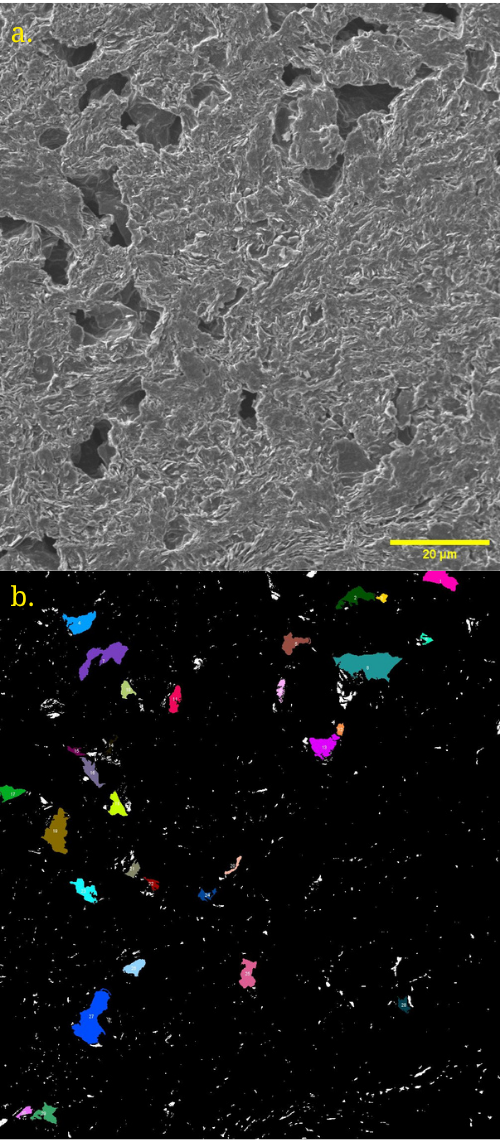
\includegraphics[width=0.45\textwidth]{./Media/C1-ig430f fused cropped 8 bit one color threshed subsample 2um areathresh}
    \caption{Draft: IG-43F subsample a. Raw and b. After intensity and pore diameter thresholding}
    \label{fig:C1-ig430f fused cropped 8 bit one color threshed subsample 2um areathresh}
\end{figure}

\subsection{Helium (He) Pycnometry}
	
Skeletal density was obtained using a Pycnomatic ATC pycnometer (Thermo Fisher
Scientific, Italy) at a temperature of 20.00 ± 0.01\textdegree{}C. Measurements
were taken in ten replicates per sample, calculating the arithmetic mean.

Solid phase volume $V_{\mathrm{SOLID}}$ was calculated assuming a theoretical
density of \todo{insert theoretical density here} g cm$^{-3}$ for an ideal
graphite crystal. Closed Pore Volume (CPV) and Open Pore Volume (OPV) for each
of the samples was calculated via equations \ref{eq:CPV} and \ref{eq:OPV}.

\begin{equation}
\mathrm{CPV} = \frac{m - V_{\mathrm{SOLID}} \times \rho{_\mathrm{s}}}{\rho{_\mathrm{s}}} 	\label{eq:CPV} 
\end{equation}

\begin{equation}
	\mathrm{OPV} = V_{\mathrm{BULK}} - \mathrm{CPV} - V_{\mathrm{SOLID}}\label{eq:OPV} 
\end{equation}

Specific Pore Volume (SPV), the void volume accessible to helium per gram of
sample was calculated via Equation \ref{eq:SPV}. 

\begin{equation}
\mathrm{SPV} = \frac{1}{\rho}-\frac{1}{\rho_\mathrm{s}}\label{eq:SPV} 
\end{equation}

\subsection{Mercury (Hg) Intrusion Porosimetry}
Mercury intrusion porosimetry operates on the fundamental principle that the
pressure at which a non-wetting fluid intrudes a given pore is inversely
proportional to the diameter of that pore (i.e., the larger the pore, the easier
it is for the non-wetting fluid to enter it). The exact physical relationship
between diameter and applied pressure is governed by the Laplace Equation (Eq.
~\ref{eq:washburn})
	
	\begin{equation} \label{eq:washburn}
		d = \frac{-4\gamma \cos \theta}{P}
	\end{equation}

		The pore diameter \(d\) is calculated using the equation:
	\begin{itemize}
		\item $d$ (m): Pore diameter
		\item $\gamma$ (N/m): Surface tension of the fluid
		\item $\theta$ (degrees): Contact angle of the fluid with the surface
		\item $Papp$ (P): Pressure
	\end{itemize}

Values of 140$^{\circ}$ and 130$^{\circ}$ were used for advancing and receding
contact angles respectively, while a value of 0.480 N m$^{-1}$ was assumed for the
surface tension of mercury \citep{VANBRAKEL19811}.  

In this work, the dataset generated by Jones et al. \citep{Jones2018} was used,
representing measurements performed not only on the same grades of graphite, but
the same batch of graphites (i.e. sampled from the same larger "brick") as those samples
which underwent SEM imaging and He pycnometry in this work.

\subsection{Nitrogen (N$_2$) Adsorption}
Low-pressure gas adsorption isotherms were obtained using a BELSORP-max
volumetric gas adsorption instrument (MicrotracBEL, Japan). 

As with mercury intrusion porosimetry, the dataset generated by Jones et al.
\citep{Jones2018} was used in this work. Once more, this represents measurements
performed on the same grades but the same batch of graphites (i.e. sampled from
the same larger "brick") as those samples which underwent SEM imaging and He
pycnometry in this work.

\section{Modelling}
PoreXpert is a void network simulation package developed at the University of
Plymouth, and now marketed worldwide by the University's spin-out company,
PoreXpert Ltd. A primary input for its modelling is the percolation
characteristic of the sample, usually measured by Hg porosimetry.  In the case
of nuclear graphite, mercury porosimeters cannot reach sufficient applied
pressure to probe the smallest voids of interest, and therefore, the percolation
characteristic is extended to smaller void sizes by Grand-Canonical Monte-Carlo
interpretation of N$_2$ adsorption.  PoreXpert is a quasi-Bayesian model which
proceeds inversely from effect (the percolation) to cause (the void network).
PoreXpert constructs an 8 dimensional parameter space,  composed of 5 numerical
parameters which represent the physical characteristics of the pore network,
such as the skew of the void (pore) size distribution, and 3 constraining
Boolean parameters, for example, to avoid structures where features overlap each
other. A Boltzmann-annealed amoeboid simplex searches over this parameter space
to find the set of parameters that produces a percolation curve minimally
different from the intrusion curve derived from Hg porosimetry and N$_2$/Kr
adsorption. The final result is a simulated pore network with the correct
porosity and percolation properties, on which many simulations, such as
pore-fluid permeability and tortuousity, and sample ageing under radiation, can
be performed \citep{MatthewsPoreXpert2025}.

\begin{figure}[!htbp]
    \centering
    \includegraphics[width=0.45\textwidth]{./Media/Modelling Pipeline.jpg.jpg}
    \caption{Full modelling pipeline, within the PoreXpert software package, integrating intrusion and SEM-derived datasets}
    \label{fig:modelling pipeline}
\end{figure}

    Modelling, conducted in PoreXpert v.3, was processed according to the
    illustrated workflow (Figure ~\ref{fig:modelling pipeline}). The user
    selects the approximation types that best reflects their interpretation of
    the depth of imaging into the porous structure (Figure
    \ref{fig:pxapproxtypes}, \citep{MatthewsPoreXpert2025}), Approximation Type
    1 \textit{Surface connected throats only} is likely to be a more accurate
    approximation for the channel porosity dataset constructed in this work, as
    a consequence of the stringent intensity threshold applied. However, due to
    stability challenges in this early compilation, approximation Type 2
    \textit{Surface connected throats and the visible volumes of connected
    pores} was applied instead (Figure ~\ref{fig:pxapproxtypes}).
    
    \todo{Without being able to run it, you could not verify, so I think it
    would be better to just specify the approximation type.}

    \begin{figure}
	    \centering
	    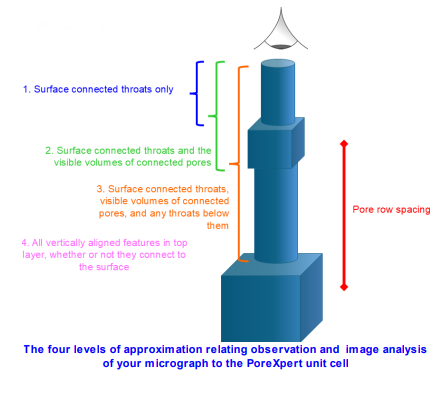
\includegraphics[width=0.45\textwidth]{./Media/PX Approximation Types.png}
	    \caption{DRAFT: Does it belong? //Approximation types available for user selection in PoreXpert v.3, selected by the user through validation based on the thresholds applied and the extent of the insight into the given media }
	    \label{fig:pxapproxtypes}
	\end{figure}

  Following the selection of parameters, the channel porosity data were entered
  into the PoreXpert v.3 interface including a minimum and maximum pore diameter
  as per (Figure ~\ref{fig:Final Workflow}),  the model was able to adjust the
  extent of the PSD which the channel porosity estimates, optimising effectively
  to a minimal distance distance of 1.91\% deviation from the experimental curve

  (Figure ~\ref{fig:PXfittinggraph})
    \begin{figure}
        \centering
        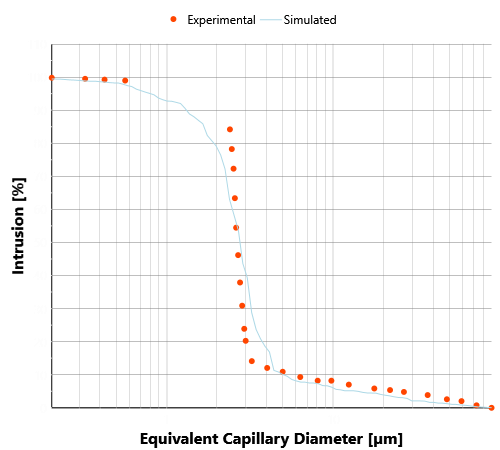
\includegraphics[width=0.45\textwidth]{./Media/Fit to percolation curve.png}
        \caption{PX Fitting process as per (Figure ~\ref{fig:modelling pipeline}). Orange dots denote experimental datapoints, the blue line is the simulated percolation curve resulting from a pore network of physically plausible parameters.}
        \label{fig:PXfittinggraph}
    \end{figure}

  The result is a pore network, upon which many simulations can be performed.
  \ref{fig:PX3dnetwork} shows a 3D rendering of the pore network generated by
  PoreXpert.

      \begin{figure}
        \centering
        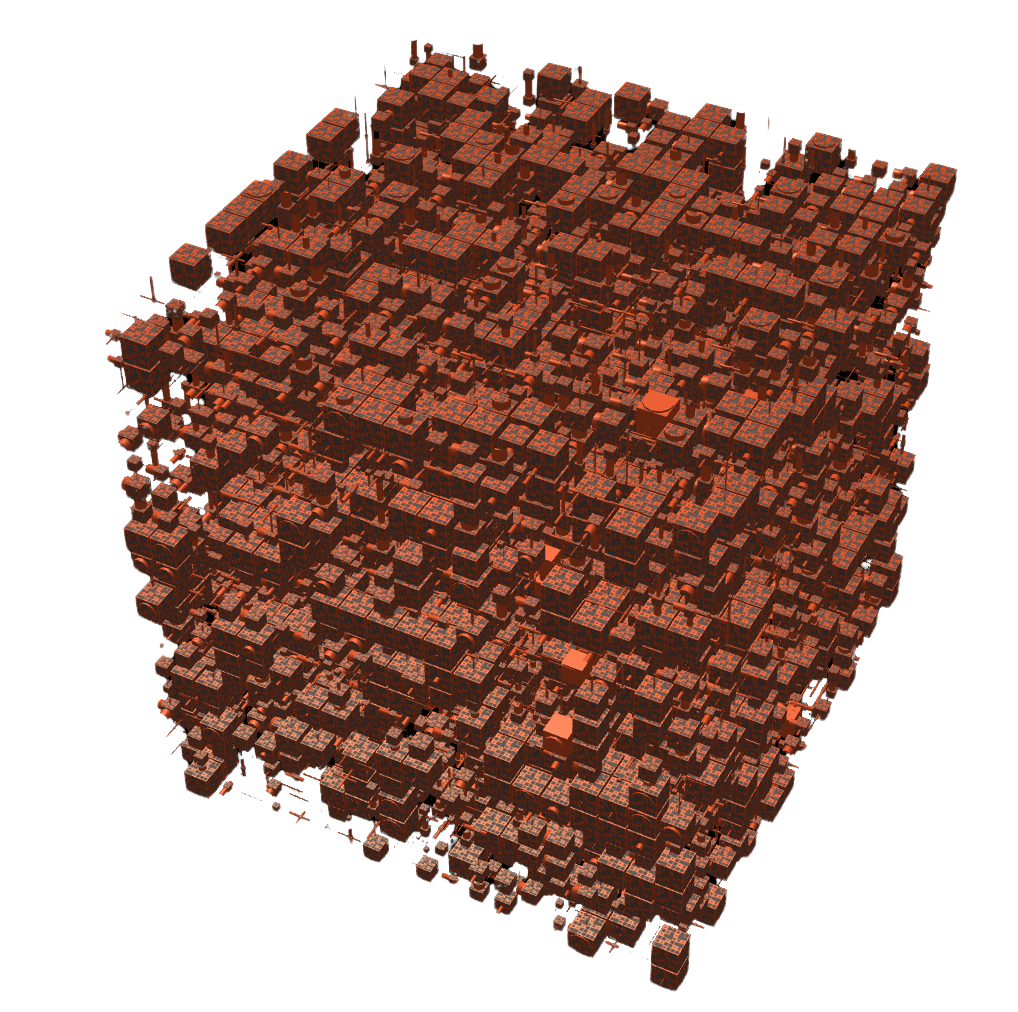
\includegraphics[width=0.45\textwidth]{./Media/unit cell no bg.png}
        \caption{PoreXpert visualisation of the pore network resulting from the
        integration of channel porosity and experimental data by the workflows
        above. 1.91\% distance between simulated and experimental curves,
        following the application of Approximation Type 2 (Figure
        ~\ref{fig:pxapproxtypes}). Channel Porosity estimation was averaged over
        the top 9 layers of a unit cell 20x20x20. The result of one generation
        of stochastic number generation. Run in Direct Mode as Batch mode
        remained unstable in this early compilation}
        \label{fig:PX3dnetwork}
    \end{figure}

    Initial testing of PoreXpert modelling demonstrate excellent congruence
    with manufacturer datasets, as exemplified below on IG-110 Sample B.
    Crucially, the linear trend line shows only a weak correlation between open
    porosity estimate and distance between simulated and experimental
    percolation characteristic (r\(^2\) = 0.32) (Figure
    \ref{fig:validationgraph}). Thus, taking the average over all stochastic
    generations of PoreXpert is a valid measure of this method's estimate of
    open porosity. 

\begin{figure}
    \centering
    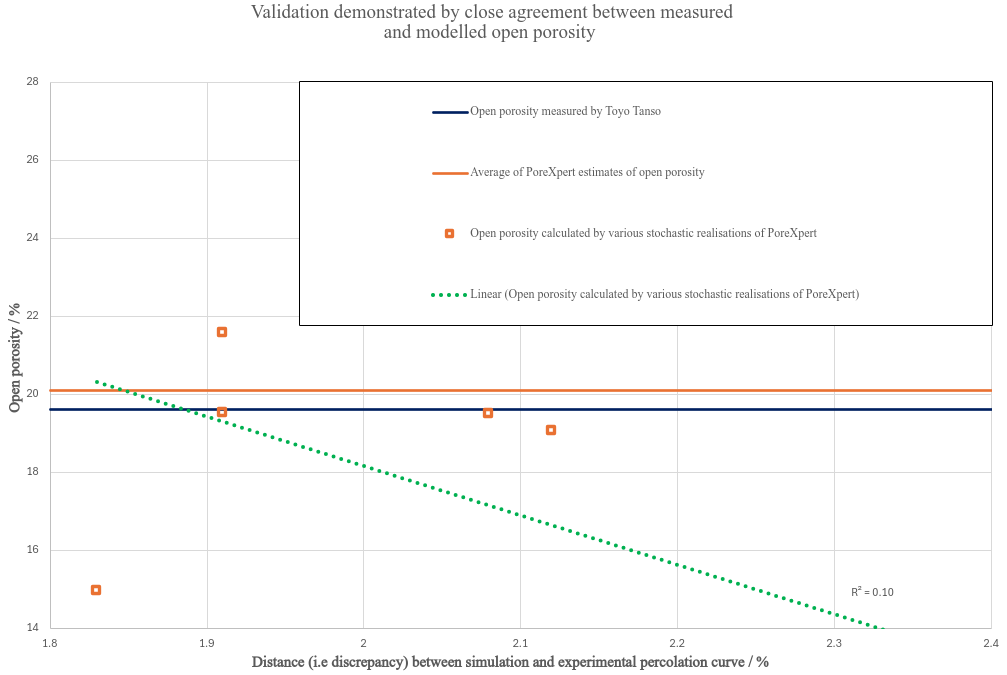
\includegraphics[width=0.45\textwidth]{./Media/ValidationGraph.png}
    \caption{DRAFT: Needs to be reformatted for publicatiom, if we choose to keep it.Validation of modelled open porosity by comparison of modelled open porosities generated by PoreXpert with manufacturer data for IG-110, which estimates a 19.62\% open porosity \cite{Jones2018}}
    \label{fig:validationgraph}
\end{figure}

  Initial modelling generated plausible data...

\section{Results}

\begin{table}
  \centering
  \caption{Pore Size Distribution (PSD) and summary characteristics for IG-110 and IG-430 samples, tabulating number of pores, total pore area, and channel porosity.}
  \label{tab:PSDtable}
  \resizebox{\columnwidth}{!}{%
    \begin{tabular}{c c c c}
      \hline
      Sample & n / pores & Total Area / $\mu$m$^2$ & Channel Porosity / \% \\
      \hline
      IG110 B & 8,684  & 41,091 & 3.14 \\
      IG110 C & 7,075  & 49,755 & 3.27 \\
      IG110 F & 8,296  & 50,735 & 3.38 \\
      IG430 B & 6,848  & 32,983 & 2.30 \\
      IG430 C & 13,026 & 49,534 & 2.94 \\
      IG430 F & 6,819  & 56,794 & 3.66 \\
      \hline
    \end{tabular}%
  }
\end{table}

The completed workflow of SEM imaging and computational composite analysis
yielded estimates of channel porosity for both graphite grades (Table
~\ref{tab:PSDtable}). IG-110 samples exhibited channel porosity values ranging
from 3.14-3.38\%, while IG-430 samples showed greater variability, ranging from
2.30-3.66\%

\begin{figure}
    \centering
    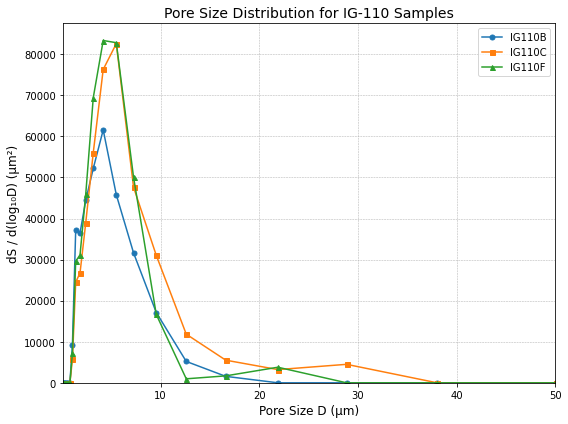
\includegraphics[width=0.45\textwidth]{./Media/IG110 ds LogD .png}
    \caption{DRAFT: I want to recheck my code on these distributions}
    \label{fig:IG110LogPSDs}
\end{figure}

\begin{figure}
    \centering
    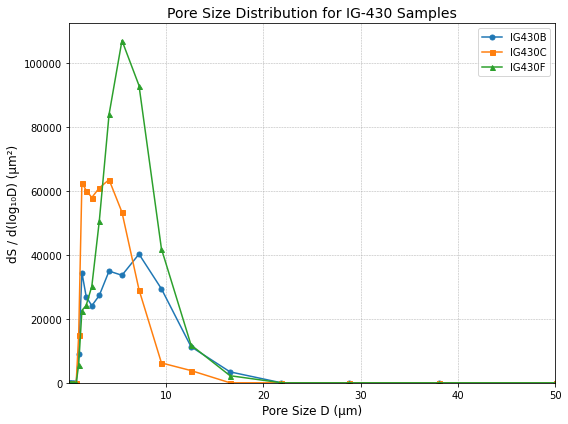
\includegraphics[width=0.45\textwidth]{./Media/IG430 ds LogD .png}
    \caption{DRAFT: I want to recheck my code on these distributions}
    \label{fig:IG430LogPSDs}
\end{figure}

Area contribution distribution is represented graphically for both graphite
grades (Figure ~\ref{fig:IG110LogPSDs}, ~\ref{fig:IG430LogPSDs}). The area of
each logarithmic bin (spanning 0.1-100 µm on the x-axis) was summed then divided
by the bin width in \(\log_{10}(D)\) to derive \(dS/d(\log_{10}D)\), with the
x-axis then linearised.  y-axis values represent area density in µm\(^2\) per
\(\log_{10}(D)\).

IG-110 and IG-430 both exhibit a peak in the sub-10 µm range. This is the
inverse of trends observed in previous OM-based analyses, where the majority of
the porosity is contributed by pores above this range \citep{Huang2019}.
\citep{huang2021statistical} found that porosity as by classified SEM, albeit 
with a different distribution, was 3\% for IG-110, which is highly
congruent with the 3.14-3.38\% range derived in this work.

Interpolation increases confidence in the basic functionality of this method.
Adjustment of the intensity threshold to match previous OM works (i.e., pore
contours and pore throats are no longer distinguished, via a reduction in
intensity threshold) produces highly similar channel porosity values.
Specifically, \citep{Kane2011a} estimated a channel porosity of 14.73\% for
IG-110, with \citep{Huang2019} deriving 14\% for the same grade, highly
congruent with the approximately 13-14\% figure this method derives with an
adjusted intensity threshold, but also illustrating the scale of the impact in
intensity threshold selection on the final channel porosity estimate.

\section{Discussion}

  \subsection{Channel Porosity Overestimation due to connecitivity algo}
  This algorithm is likely to yield at least a  slight overestimation of the
channel porosity. This is because such an inclusive definition means that two or
more pores, connected by a narrow neck or even simply with adjacent pixels,
would be classified as a single pore. Notably, this would not change the final
channel porosity (\%), at least in isolation, but would result in a rightward
shift in the PSD. Skeleton segmentation is for fine-grade nuclear graphite
likely to be a more accurate approach than a simple connectivity algorithm as
used here would be a key improvement if implemented
\cite{ARREGUIMENA2022112047}

\subsection{Pore Fragmentation and Implications for Modelling}
The application of a maximum pore diameter is a key part of the modelling as
  initial modelling where this was not implemented failed to yield reliable
  results. It is believed that this is due to the impossiblity of the model
  fitting an plausible network on the premise that pores from 1.12 um diameter
  upwards represent only 3 \% of the sample surface. Imposing an upper threshold
  as the simple max of the pore diameters identified by SEM is an uncomplicated
  initial solution which has more logical implications (i.e., to state that
  between 1.12 and 20um diameter, 3\% of the sample surface is represented by
  porosity). This threshold varied between 13-26 um in this work, which should
  cover the vast majority of the porosity, particularly given the pore fragmentation
  issue described below.

  Specifically, the use of a simple Moore neighbourhood connectivity, when
  combined with the fact that Erosion and Dilation binary operations were not
  applied, means that pores which the operator identifies as a single pore are
  in more than one case instead defined as two or more pores. Not only this but
  these split pores may not then surpass the pore diameter threshold of 1.12um.
  (e.g., a pore of 10um diameter might be split into 2 pores, 1 of 9um diameter
  and another of 1um diameter, which would be discarded due to the pore diameter
  threshold, reducing the channel porosity \% and shifting rightward the pore
  size distribution).

  The end result is that it is difficult to describe the pore size distribution
  derived from SEM as it currently stands, as completely impenetrable.
  Crucially, the production of reasonable results from the modelling as above
  depends on an accurate constraint of the pore diameter interval (i.e., the
  channnel porosity figure of 3\% refers only to porosity between 1.12 and 25um
  diameter) and so not only the SEM-derived pore size distribution but the PX
  modelling which uses it, has at least some reduction in reliability due to the
  pore fragmentation issue. However, this is likely a soluble problem, as follows.

  \subsection{Proposed Future Workflow}

  -Just my idea of an improved workflow:
  1. Resin Impregnation
  2. SEM (see if we can go to 2kV)
  3. Otsu Thresholding (We have clear bimodality thanks to Resin impregnation)
  4. Skeleton segmentation (Avizo software needed?)
  5. Apply improved pore diameter thresholds, or maybe do not do any at all as no longer needed? At least lowered.
  6. Modelling


\clearpage

\bibliography{bibliography}
\end{document}